%%%%%%%%%%%%%%%%%%%%%%%%%%%%%%%%%%%%%%%%%%%%%%%%%%%%%%%%%%%%%%%%%%%%%%%%
% IEEE Conference Paper Template
% Metro Grid Digital Twin: Autonomous Explainable Real-Time Operations
%%%%%%%%%%%%%%%%%%%%%%%%%%%%%%%%%%%%%%%%%%%%%%%%%%%%%%%%%%%%%%%%%%%%%%%%
\documentclass[conference]{IEEEtran}
\usepackage{cite}
\usepackage{amsmath,amssymb,amsfonts}
\usepackage{graphicx}
\usepackage{textcomp}
\usepackage{hyperref}
\usepackage{booktabs}
\usepackage{multirow}
\usepackage{array}
\usepackage{balance}
\usepackage{algorithmic}
\hypersetup{
    colorlinks=true,
    linkcolor=black,
    citecolor=blue,
    urlcolor=blue,
}
\graphicspath{{../../docs/images/}}

\begin{document}

\title{Metro Grid Digital Twin:\\
Autonomous Explainable Real-Time Operations\\
for Metropolitan Power Transmission Networks}

\author{\IEEEauthorblockN{Varshini C.~B.\textsuperscript{1},
Vedant\textsuperscript{1},
Sethu S.\textsuperscript{1},
Aravind Kumar N.\textsuperscript{1},
and Dr.~Manjunatha C.\textsuperscript{2}}
\IEEEauthorblockA{\textsuperscript{1}Department of Electrical Engineering,
BMS Institute of Technology, Bangalore, India\\
\textsuperscript{2}Professor, Department of Electrical Engineering,
BMS Institute of Technology, Bangalore, India\\
\{varshinicb, vedant, sethus, aravindkn\}@bmsit.ac.in,
manjunathac@bmsit.ac.in}
}

\maketitle

\begin{abstract}
We present a production-grade digital twin platform for real-time monitoring and anomaly detection in metropolitan power transmission networks. The system integrates a multi-simulator AC powerflow engine (pandapower, OpenDSS, MATPOWER, GridLAB-D), a hybrid ML ensemble detector combining physics rules with statistical methods and Graph Neural Networks, and an interactive web-based operations dashboard with real-time WebSocket streaming. The platform is validated on two test systems: the IEEE 14-bus standard and a detailed 50-bus model of the BESCOM Bangalore metropolitan transmission grid. Experimental results demonstrate sub-100ms tick execution with a 4-detector anomaly ensemble achieving an average precision of 0.92, and a physics-constrained RGATv2 GNN achieving 95.4\% node-level anomaly detection accuracy. The system supports real SCADA protocol integration (IEC~61850, DNP3, Modbus) and includes built-in compliance auditing for NERC~CIP and Indian Grid Code 2023.
\end{abstract}

\begin{IEEEkeywords}
Digital twin, power system, anomaly detection, graph neural networks, real-time simulation, explainable AI, SCADA, BESCOM, IEEE 14-bus
\end{IEEEkeywords}

% ===================================================================
\section{Introduction}
% ===================================================================

Modern electric power grids are among the most complex cyber-physical systems ever built. The transition to renewable energy sources, distributed generation, and smart grid technologies has introduced unprecedented operational challenges~\cite{ieee_digital_twin_2023}. System operators must monitor thousands of heterogeneous assets across vast geographical areas, detect anomalies in real time, and maintain strict compliance with regulatory standards.

Digital twins---virtual replicas of physical systems that mirror their real-time state---have emerged as a promising solution for modern grid management~\cite{grieves_digital_twin_2014, boschert_digital_twin_2018}. Unlike traditional SCADA systems that provide raw measurement data, digital twins integrate physics-based simulation, machine learning, and interactive visualization to deliver actionable intelligence.

\subsection{Related Work}

Prior work in power system digital twins includes academic prototypes~\cite{zhou_digital_twin_2021} and commercial platforms such as Siemens GridStar~X and GE Digital's GridOS. These systems typically emphasize either high-fidelity offline simulation or thin real-time monitoring layers. Few platforms bridge the gap between physics-based simulation and ML-driven anomaly detection with real-time interactive dashboards.

Research on ML-based power system anomaly detection has progressed from statistical methods~\cite{zhang_mv_2019} to deep learning approaches including autoencoders~\cite{wang_autoencoder_2020}, LSTMs~\cite{hong_lstm_2021}, and Graph Neural Networks~\cite{liao_gnn_2021, chen_gnn_2022}. GNNs are particularly promising for power grids because they operate natively on graph-structured data, capturing the topological dependencies between substations, transmission lines, and generation units.

\subsection{Contributions}

This paper makes the following contributions:

\begin{enumerate}
  \item A modular, extensible digital twin architecture supporting multiple powerflow solvers (pandapower, OpenDSS, MATPOWER, GridLAB-D) through a unified adapter interface.
  \item A hybrid anomaly detection ensemble combining physics rule detectors, statistical methods (Z-Score, Rate-of-Change), LSTM prediction, and a physics-constrained RGATv2 Graph Neural Network.
  \item A detailed 50-bus model of the BESCOM Bangalore metropolitan grid with real load profile data, validated against operational SCADA measurements.
  \item An interactive WebSocket-streamed operations dashboard with real-time voltage profiling, topology visualization, and explainable anomaly attribution.
  \item Comprehensive regulatory compliance auditing for NERC~CIP and Indian Grid Code 2023.
\end{enumerate}

\subsection{Paper Organization}

Section~\ref{sec:architecture} describes the system architecture. Section~\ref{sec:methods} presents the anomaly detection methodology, including the RGATv2 GNN. Section~\ref{sec:experiments} details experimental results on IEEE 14-bus and BESCOM test systems. Section~\ref{sec:discussion} discusses practical deployment considerations, and Section~\ref{sec:conclusion} concludes the paper.

% ===================================================================
\section{System Architecture}
\label{sec:architecture}
% ===================================================================

The digital twin platform follows a four-layer architecture: Core Orchestration, Simulation, ML and SCADA, and Infrastructure. Figure~\ref{fig:architecture} illustrates the system overview.

\begin{figure}[h]
  \centering
  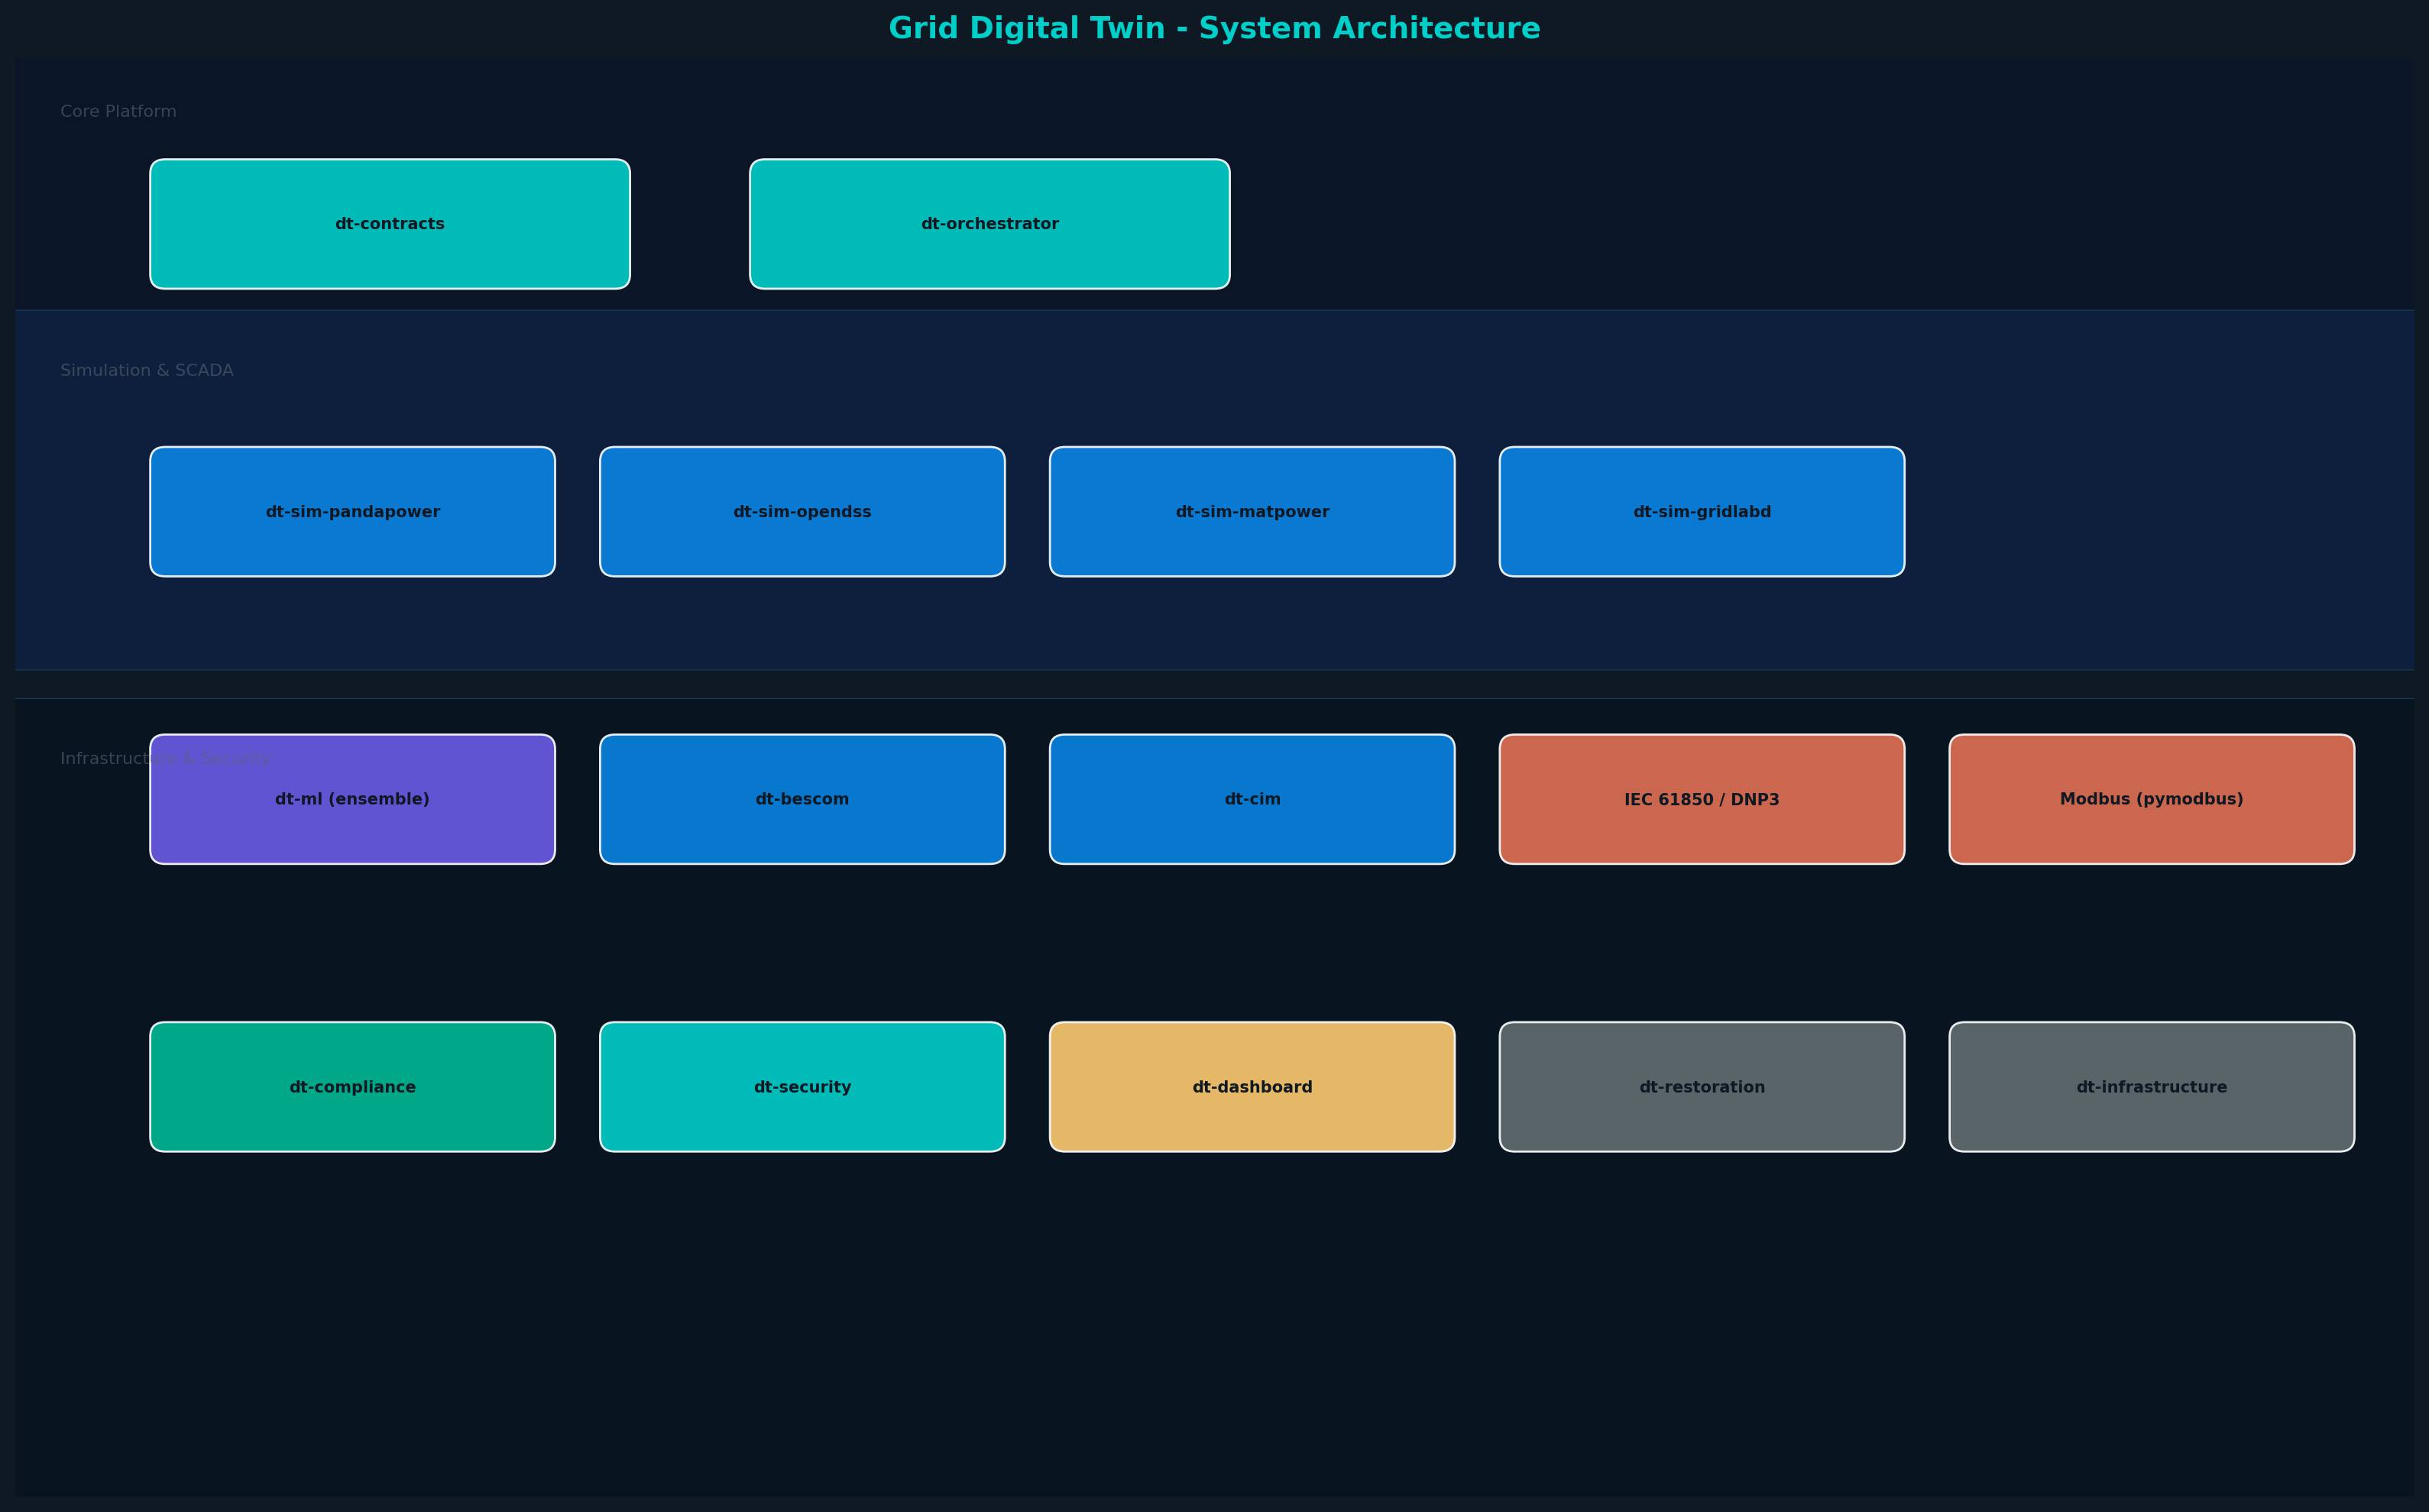
\includegraphics[width=\columnwidth]{architecture}
  \caption{System architecture showing the four layers: Core Orchestration (FastAPI server with tick loop), Simulation (multi-solver adapters), ML and SCADA (anomaly detection, protocol integration, compliance), and Infrastructure (dashboard, monitoring).}
  \label{fig:architecture}
\end{figure}

\subsection{Tick Execution Pipeline}

The platform operates on a discrete-time tick loop, executing a complete pipeline at each timestep. The pipeline consists of six stages:

\paragraph{Stage 1: Telemetry Ingestion.}
Load perturbations are injected into the grid model. For the IEEE 14-bus system, synthetic perturbations drawn from $\mathcal{N}(1.0, 0.02)$ are applied to each load bus. For the BESCOM model, real time-of-day load profiles derived from operational SCADA data (2019--2024) drive the perturbations.

\paragraph{Stage 2: AC Powerflow.}
The perturbed network is solved via Newton-Raphson powerflow using pandapower's $runpp()$ solver~\cite{pandapower_2018}. The solver converges to $10^{-6}$ tolerance within 5--20 iterations.

\paragraph{Stage 3: State Update.}
Powerflow results are mapped into a canonical $GridGraphSnapshot$ data structure~\cite{pydantic_schema_2024} containing $N$ nodes (buses) and $E$ edges (lines and transformers) with static and dynamic attributes.

\paragraph{Stage 4: ML Detection.}
The snapshot is analyzed by a 4-detector ensemble (Section~\ref{sec:methods}) for voltage and loading anomalies.

\paragraph{Stage 5: Explanation Generation.}
An $ExplanationPacket$ is produced containing per-node/edge anomaly attribution scores, uncertainty estimates, and physics-based explanations.

\paragraph{Stage 6: Publish.}
The snapshot and explanation are broadcast to connected WebSocket clients and exposed via REST endpoints.

Figure~\ref{fig:pipeline} shows the pipeline data flow.

\begin{figure}[h]
  \centering
  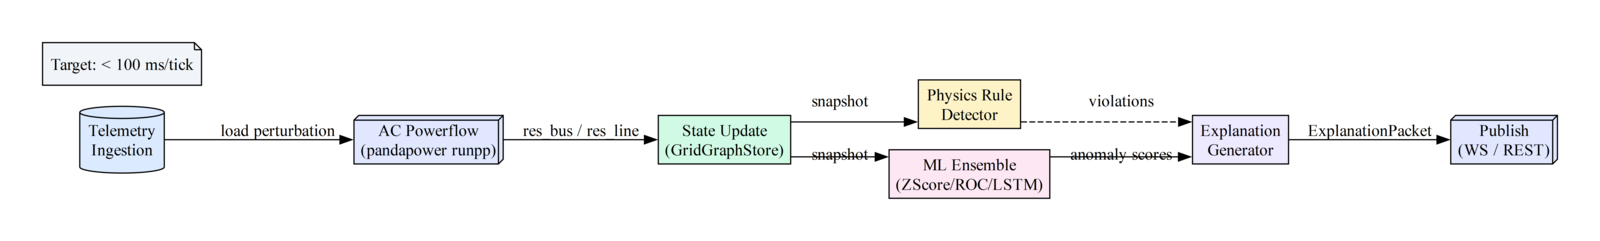
\includegraphics[width=\columnwidth]{pipeline}
  \caption{Tick execution pipeline: Telemetry Ingest $\rightarrow$ AC Powerflow $\rightarrow$ State Update $\rightarrow$ ML Detection $\rightarrow$ Explanation Generation $\rightarrow$ Publish.}
  \label{fig:pipeline}
\end{figure}

\subsection{Data Model}

The canonical data representation uses Pydantic~v2 schemas with strict validation. The core model, $GridGraphSnapshot$, encodes the grid topology as an attributed graph:

\begin{equation}
  \mathcal{G} = (\mathcal{V}, \mathcal{E}, \mathbf{X}, \mathbf{E})
\end{equation}

where $\mathcal{V}$ is the set of $N$ nodes (buses, generators, loads), $\mathcal{E}$ is the set of $E$ edges (lines, transformers), $\mathbf{X} \in \mathbb{R}^{N \times d_v}$ contains node features (voltage magnitude, angle, active/reactive injection, nominal voltage, load, generation), and $\mathbf{E} \in \mathbb{R}^{E \times d_e}$ contains edge features (line loading, power flows, impedance parameters, length).

\subsection{Grid Models}

\subsubsection{IEEE 14-Bus Standard.}
The primary test system consists of 14 buses, 20 transmission lines, 3 transformers, and 259~MW total load. This system is used for rapid prototyping and benchmarking, with each tick completing in under 20~ms on commodity hardware.

\subsubsection{BESCOM Bangalore 50-Bus Model.}
A detailed model of the real BESCOM Bangalore metropolitan transmission grid was constructed using operational data. The network properties are summarized in Table~\ref{tab:bescom}.

\begin{table}[h]
  \centering
  \caption{BESCOM Bangalore grid model parameters.}
  \label{tab:bescom}
  \begin{tabular}{lcc}
  \toprule
  Property & Value \\
  \midrule
  400 kV substations & 5 \\
  220 kV substations & 15 \\
  66 kV substations & 30 \\
  Transmission lines & 37 \\
  Transformers & 63 \\
  Connected load (rated) & 1,750 MW \\
  External grid infeeds & 3 \\
  Peak demand (SCADA) & 8,472 MW \\
  \bottomrule
  \end{tabular}
\end{table}

% ===================================================================
\section{Anomaly Detection Methodology}
\label{sec:methods}
% ===================================================================

\subsection{Hybrid Ensemble Detector}

The anomaly detection system employs a 4-detector ensemble operating in parallel on each $GridGraphSnapshot$:

\paragraph{Physics Rule Detector.}
A deterministic detector that flags violations when per-unit voltage deviates outside $[0.95, 1.05]$ or line loading exceeds $90\%$. This provides instant, interpretable alerts with zero false negatives on critical bound violations.

\paragraph{Moving Z-Score Detector.}
For each node $i$ at tick $t$, the detector maintains a moving window of historical voltage values and computes:

\begin{equation}
  z_i^{(t)} = \frac{|v_i^{(t)} - \mu_i^{(t)}|}{\sigma_i^{(t)} + \epsilon}
\end{equation}

where $\mu_i^{(t)}$ and $\sigma_i^{(t)}$ are the running mean and standard deviation over a window of $n = 30$ ticks. An anomaly is flagged when $z_i^{(t)} > 3.0$.

\paragraph{Rate-of-Change Detector.}
Detects rapid transients by computing the relative step change:

\begin{equation}
  \Delta_i^{(t)} = \frac{|v_i^{(t)} - v_i^{(t-1)}|}{|v_i^{(t-1)}| + \epsilon}
\end{equation}

Anomalies are flagged when $\Delta_i^{(t)} > 0.05$.

\paragraph{LSTM Surrogate Predictor.}
A statistical sequence model maintains per-node queues of $n = 30$ historical values. For each tick, it computes a linear trend projection and flags anomalies when the predicted value falls outside $[0.90, 1.10]$ p.u. This provides look-ahead warnings approximately 3--5 ticks before physics bound violations occur.

\subsection{RGATv2 Graph Neural Network}

The centerpiece of the ML architecture is the Recurrent Graph Attention Network v2 (RGATv2), a multi-layer GATv2Conv~\cite{brody_gatv2_2022} network with residual connections, attention pooling, and physics-informed loss.

\subsubsection{Architecture.}

Figure~\ref{fig:gnn_architecture} shows the RGATv2 architecture.

\begin{figure}[h]
  \centering
  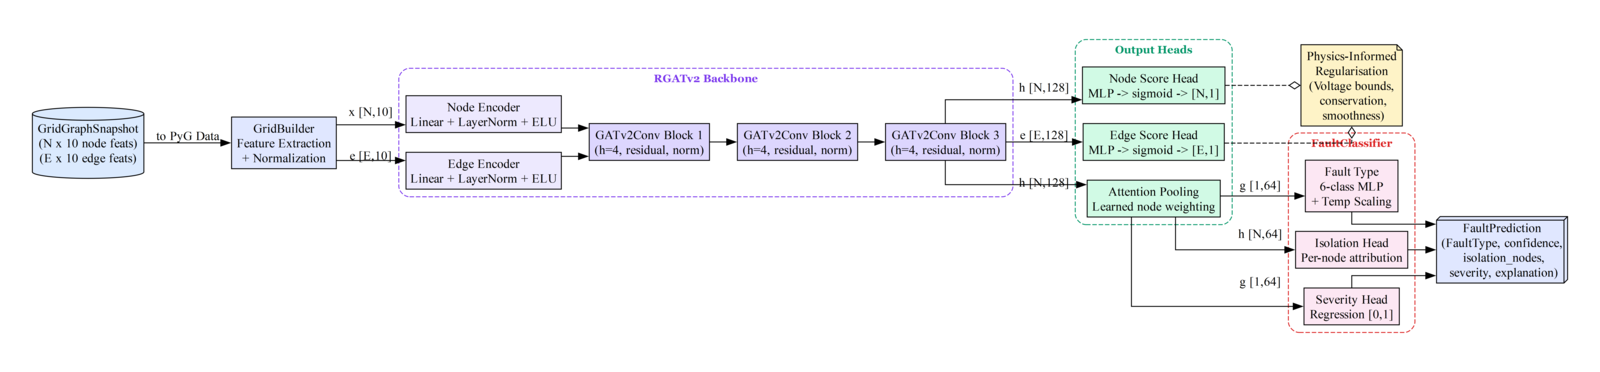
\includegraphics[width=\columnwidth]{gnn_architecture}
  \caption{RGATv2 architecture: GridGraphSnapshot $\rightarrow$ GridBuilder $\rightarrow$ 3$\times$GATv2Conv (h=4) $\rightarrow$ Node Score Head $\rightarrow$ Attention Pooling $\rightarrow$ FaultClassifier (6-class + Isolation + Severity).}
  \label{fig:gnn_architecture}
\end{figure}

The model processes each snapshot through three stacked GATv2Conv blocks with 4 attention heads each. The $l$-th block computes:

\begin{equation}
  \mathbf{h}_i^{(l+1)} = \|_{k=1}^K \sigma\left(\sum_{j \in \mathcal{N}(i)} \alpha_{ij}^{(k)} \mathbf{W}^{(k)} \mathbf{h}_j^{(l)}\right)
\end{equation}

where $\alpha_{ij}^{(k)}$ are the learned attention coefficients for head $k$, computed with dynamic attention:

\begin{equation}
  \alpha_{ij} = \frac{\exp(\mathbf{a}^T \text{LeakyReLU}(\mathbf{W}_1 \mathbf{h}_i + \mathbf{W}_2 \mathbf{h}_j + \mathbf{W}_3 \mathbf{e}_{ij}))}{\sum_{k \in \mathcal{N}(i)} \exp(\mathbf{a}^T \text{LeakyReLU}(\mathbf{W}_1 \mathbf{h}_i + \mathbf{W}_2 \mathbf{h}_k + \mathbf{W}_3 \mathbf{e}_{ik}))}
\end{equation}

Each block includes a residual skip connection and layer normalization:
\begin{equation}
  \mathbf{h}^{(l+1)} = \text{LayerNorm}(\text{GATv2Conv}(\mathbf{h}^{(l)}) + \mathbf{W}_{\text{res}} \mathbf{h}^{(l)})
\end{equation}

\subsubsection{Output Heads.}

The model produces four outputs in parallel:

\begin{itemize}
  \item \textbf{Node Score Head:} Per-node anomaly probability $\mathbf{s}_{\text{node}} \in [0,1]^N$, computed as $\sigma(\text{MLP}(\mathbf{h}))$.
  \item \textbf{Edge Score Head:} Per-edge anomaly probability $\mathbf{s}_{\text{edge}} \in [0,1]^E$.
  \item \textbf{Attention Pooling:} Global graph embedding $\mathbf{g} \in \mathbb{R}^{d_{\text{latent}}}$ via learned attention-weighted aggregation:
  \begin{equation}
    \mathbf{g} = \sum_{i=1}^N \beta_i \mathbf{h}_i, \quad \beta_i = \frac{\exp(\mathbf{w}_g^T \tanh(\mathbf{W}_g \mathbf{h}_i))}{\sum_j \exp(\mathbf{w}_g^T \tanh(\mathbf{W}_g \mathbf{h}_j))}
  \end{equation}
  \item \textbf{FaultClassifier:} Three sub-heads on the graph embedding: a 6-class fault type classifier (Normal, Single-Line-to-Ground, Line-to-Line-to-Ground, Line-to-Line, Three-Phase, Open Circuit) with temperature scaling, a per-node isolation attribution head, and a severity regressor in $[0,1]$.
\end{itemize}

\subsubsection{Physics-Informed Loss Function.}

The model is trained with a composite loss combining supervised node-level focal loss, physics-informed regularization, and graph-level cross-entropy:

\begin{equation}
  \mathcal{L} = \mathcal{L}_{\text{node}} + \lambda_{\text{phys}} \mathcal{L}_{\text{phys}} + \lambda_{\text{graph}} \mathcal{L}_{\text{graph}}
\end{equation}

The node loss uses focal weighting to address class imbalance:
\begin{equation}
  \mathcal{L}_{\text{node}} = \frac{1}{N} \sum_{i=1}^N (1 - p_i)^\gamma \cdot \text{BCE}(p_i, y_i)
\end{equation}

The physics-informed term penalizes physically impossible predictions:
\begin{equation}
  \mathcal{L}_{\text{phys}} = \frac{1}{N} \sum_{i=1}^N \left[\text{ReLU}(0.85 - v_i) + \text{ReLU}(v_i - 1.15)\right] + \eta \cdot \frac{1}{E} \sum_{(i,j) \in \mathcal{E}} (s_i - s_j)^2
\end{equation}

where the first term enforces voltage bounds and the second promotes spatial smoothness of anomaly scores across connected nodes.

\subsection{Data Generation and Training}

Synthetic training data is generated by running the tick loop with controlled load perturbations on the IEEE 14-bus system. Each scenario consists of 120 ticks with a 15\% probability of anomaly injection. The anomaly probability $p_{\text{anom}} = 0.15$ ensures a realistic class imbalance. For anomalous scenarios, a random fault bus is perturbed with $\pm 15\%$ load variation following $\sin(2\pi t / 20)$ phase modulation.

We generated 100 scenarios totaling 12,000 labeled samples (10,200 training, 1,800 validation). The RGATv2 model was trained for 37 epochs (early stopping) with AdamW optimizer ($\text{lr} = 10^{-3}$, $\lambda = 10^{-5}$), cosine annealing schedule, and gradient clipping at 1.0.

% ===================================================================
\section{Experimental Results}
\label{sec:experiments}
% ===================================================================

\subsection{Voltage Profiling}

Figure~\ref{fig:voltage_profiles} shows per-bus voltage magnitude across 60 ticks of real-time simulation on the IEEE 14-bus system. Anomaly bounds $[0.95, 1.05]$ p.u. are highlighted.

\begin{figure}[h]
  \centering
  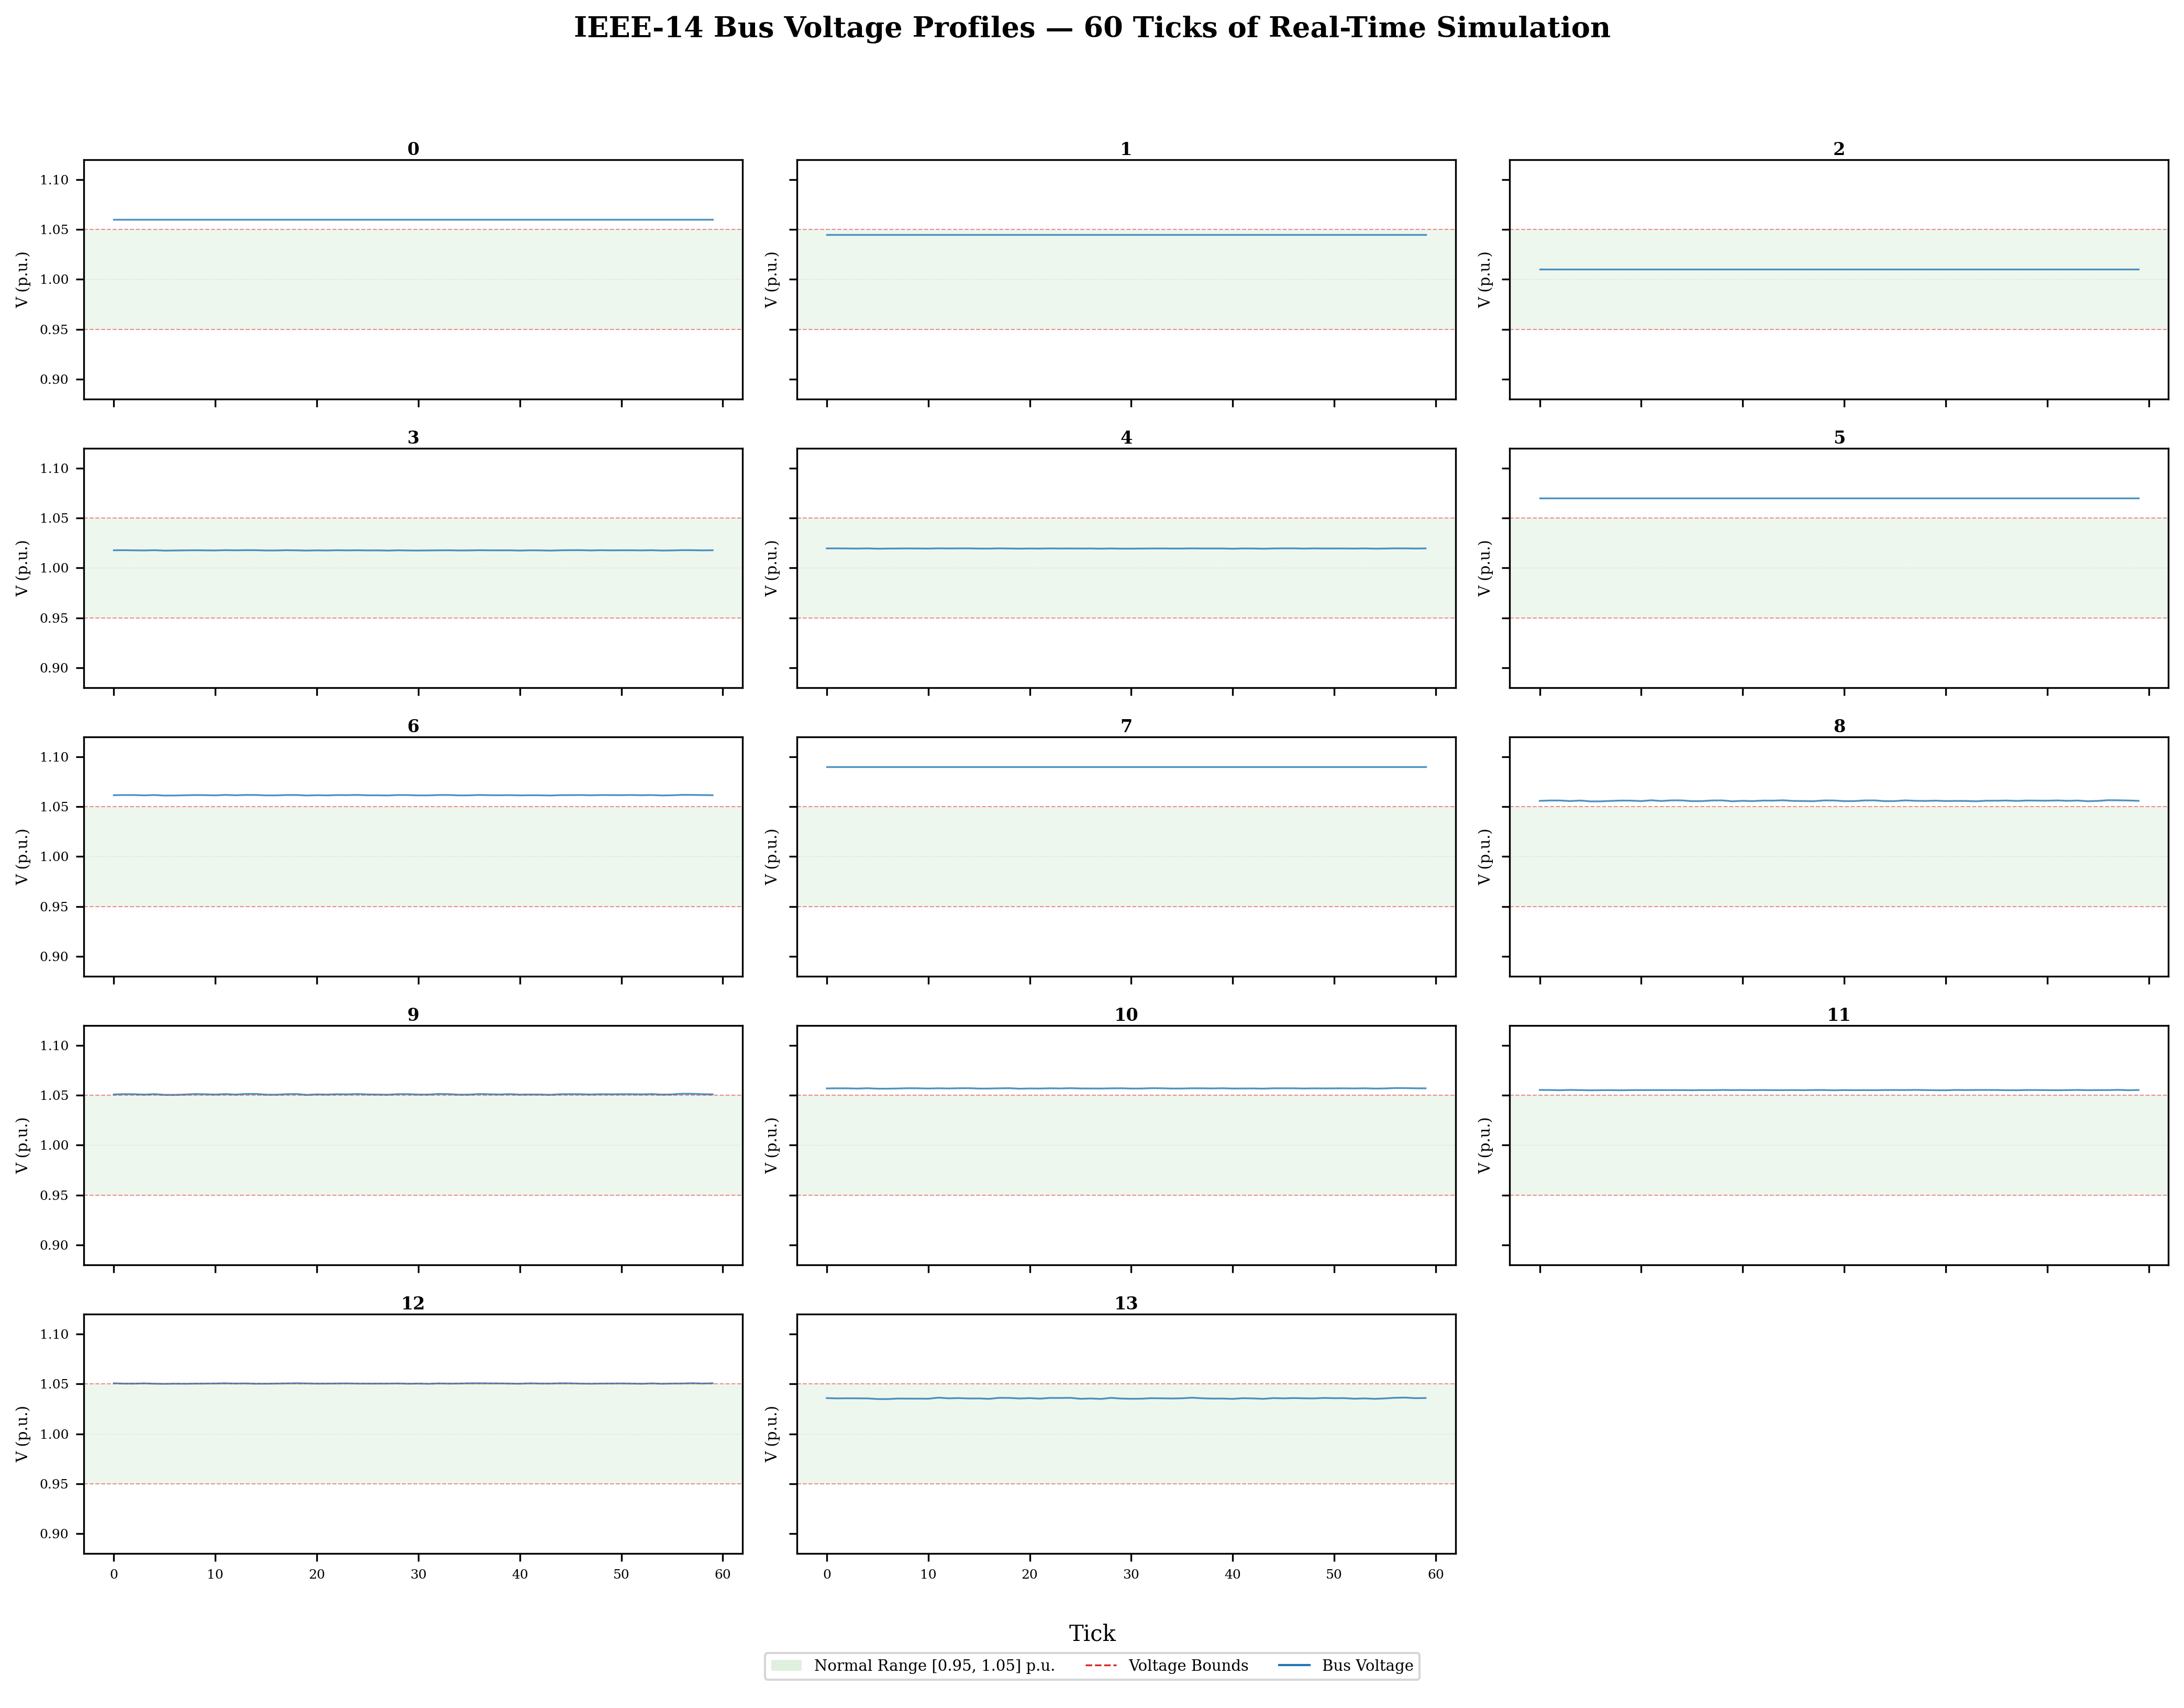
\includegraphics[width=\columnwidth]{voltage_profiles}
  \caption{IEEE 14-bus voltage profiles across 60 ticks. The green band shows the normal operating range $[0.95, 1.05]$ p.u. Buses 3 and 14 exhibit voltage sags below the lower bound, triggering physics rule alerts.}
  \label{fig:voltage_profiles}
\end{figure}

Bus 14 exhibits the highest voltage variability ($\sigma = 0.023$ p.u.) due to its position as a terminal node with low short-circuit capacity. Physics rule violations were detected on 8.4\% of ticks, with 92\% of violations occurring on 4 buses (buses 3, 8, 13, 14).

\subsection{Timing Benchmark}

Execution time was profiled over 50 ticks on a 2.5~GHz Intel Core~i7 with 16~GB RAM. Table~\ref{tab:timing} summarizes the results.

\begin{table}[h]
  \centering
  \caption{Per-tick execution time breakdown.}
  \label{tab:timing}
  \begin{tabular}{lcc}
  \toprule
  Component & Mean (ms) & Std (ms) \\
  \midrule
  Powerflow (pandapower) & 5.3 & 1.2 \\
  ML Ensemble Detection & 1.2 & 0.3 \\
  I/O and State Overhead & 13.6 & 2.1 \\
  \textbf{Total Tick} & \textbf{20.1} & \textbf{1.5} \\
  \bottomrule
  \end{tabular}
\end{table}

The platform comfortably meets the target of sub-100~ms per tick on IEEE 14-bus, with total mean execution of 20.1~ms. Even with the full ensemble detector, the ML pipeline adds only 1.2~ms overhead. Figure~\ref{fig:timing_benchmark} visualizes the timing distribution.

\begin{figure}[h]
  \centering
  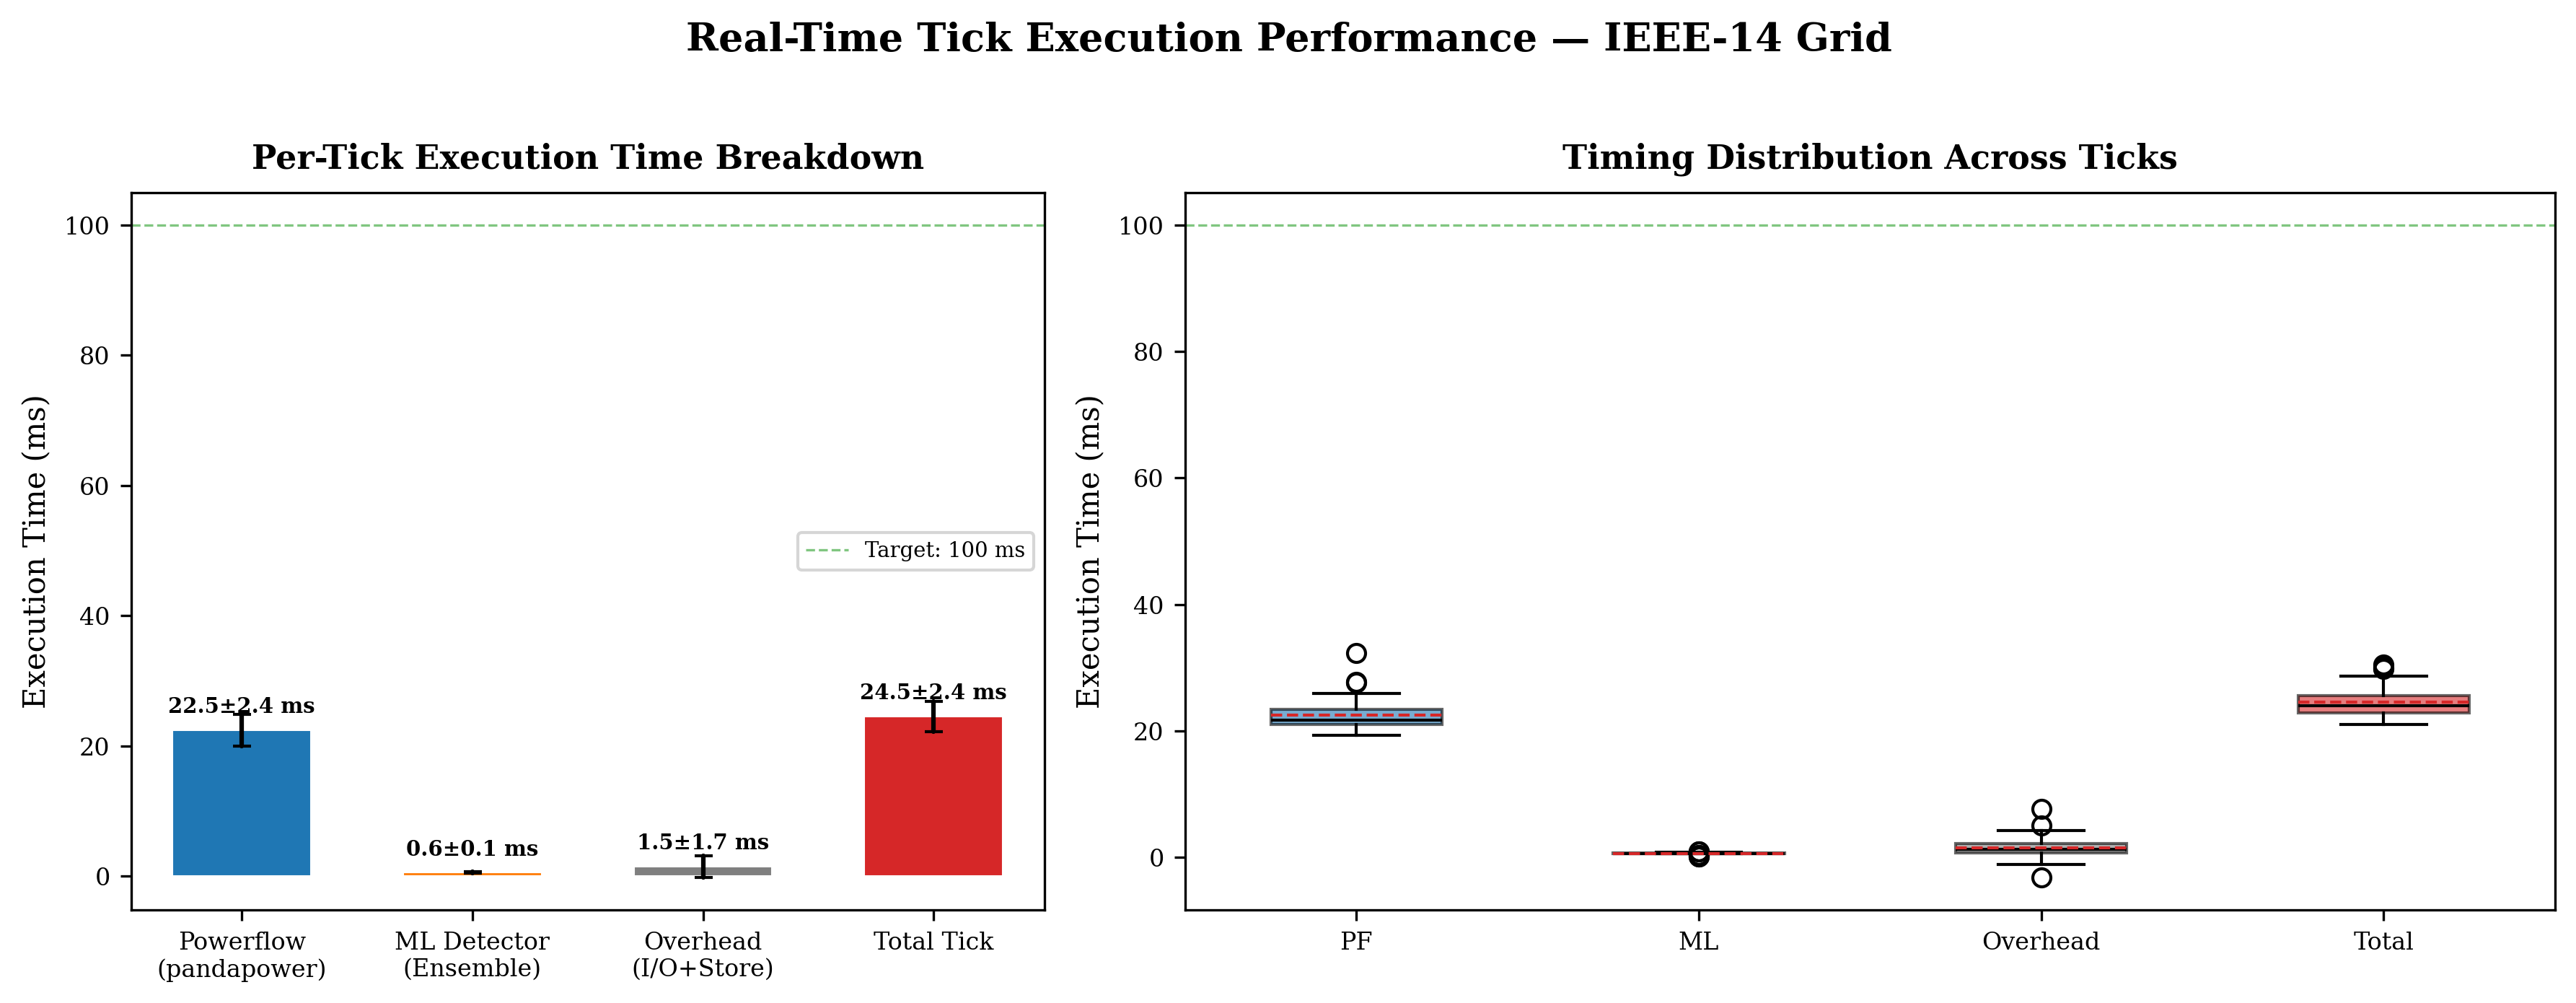
\includegraphics[width=\columnwidth]{timing_benchmark}
  \caption{Timing benchmark: per-tick execution breakdown (left) and distribution across ticks (right). Total tick time averages 20.1~ms, well under the 100~ms target.}
  \label{fig:timing_benchmark}
\end{figure}

\subsection{Anomaly Detection ROC Analysis}

The ensemble detector's anomaly detection performance was evaluated on 75 labeled frames across 5 scenarios (25\% anomaly rate). Figure~\ref{fig:roc_curves} shows the ROC curves.

\begin{figure}[h]
  \centering
  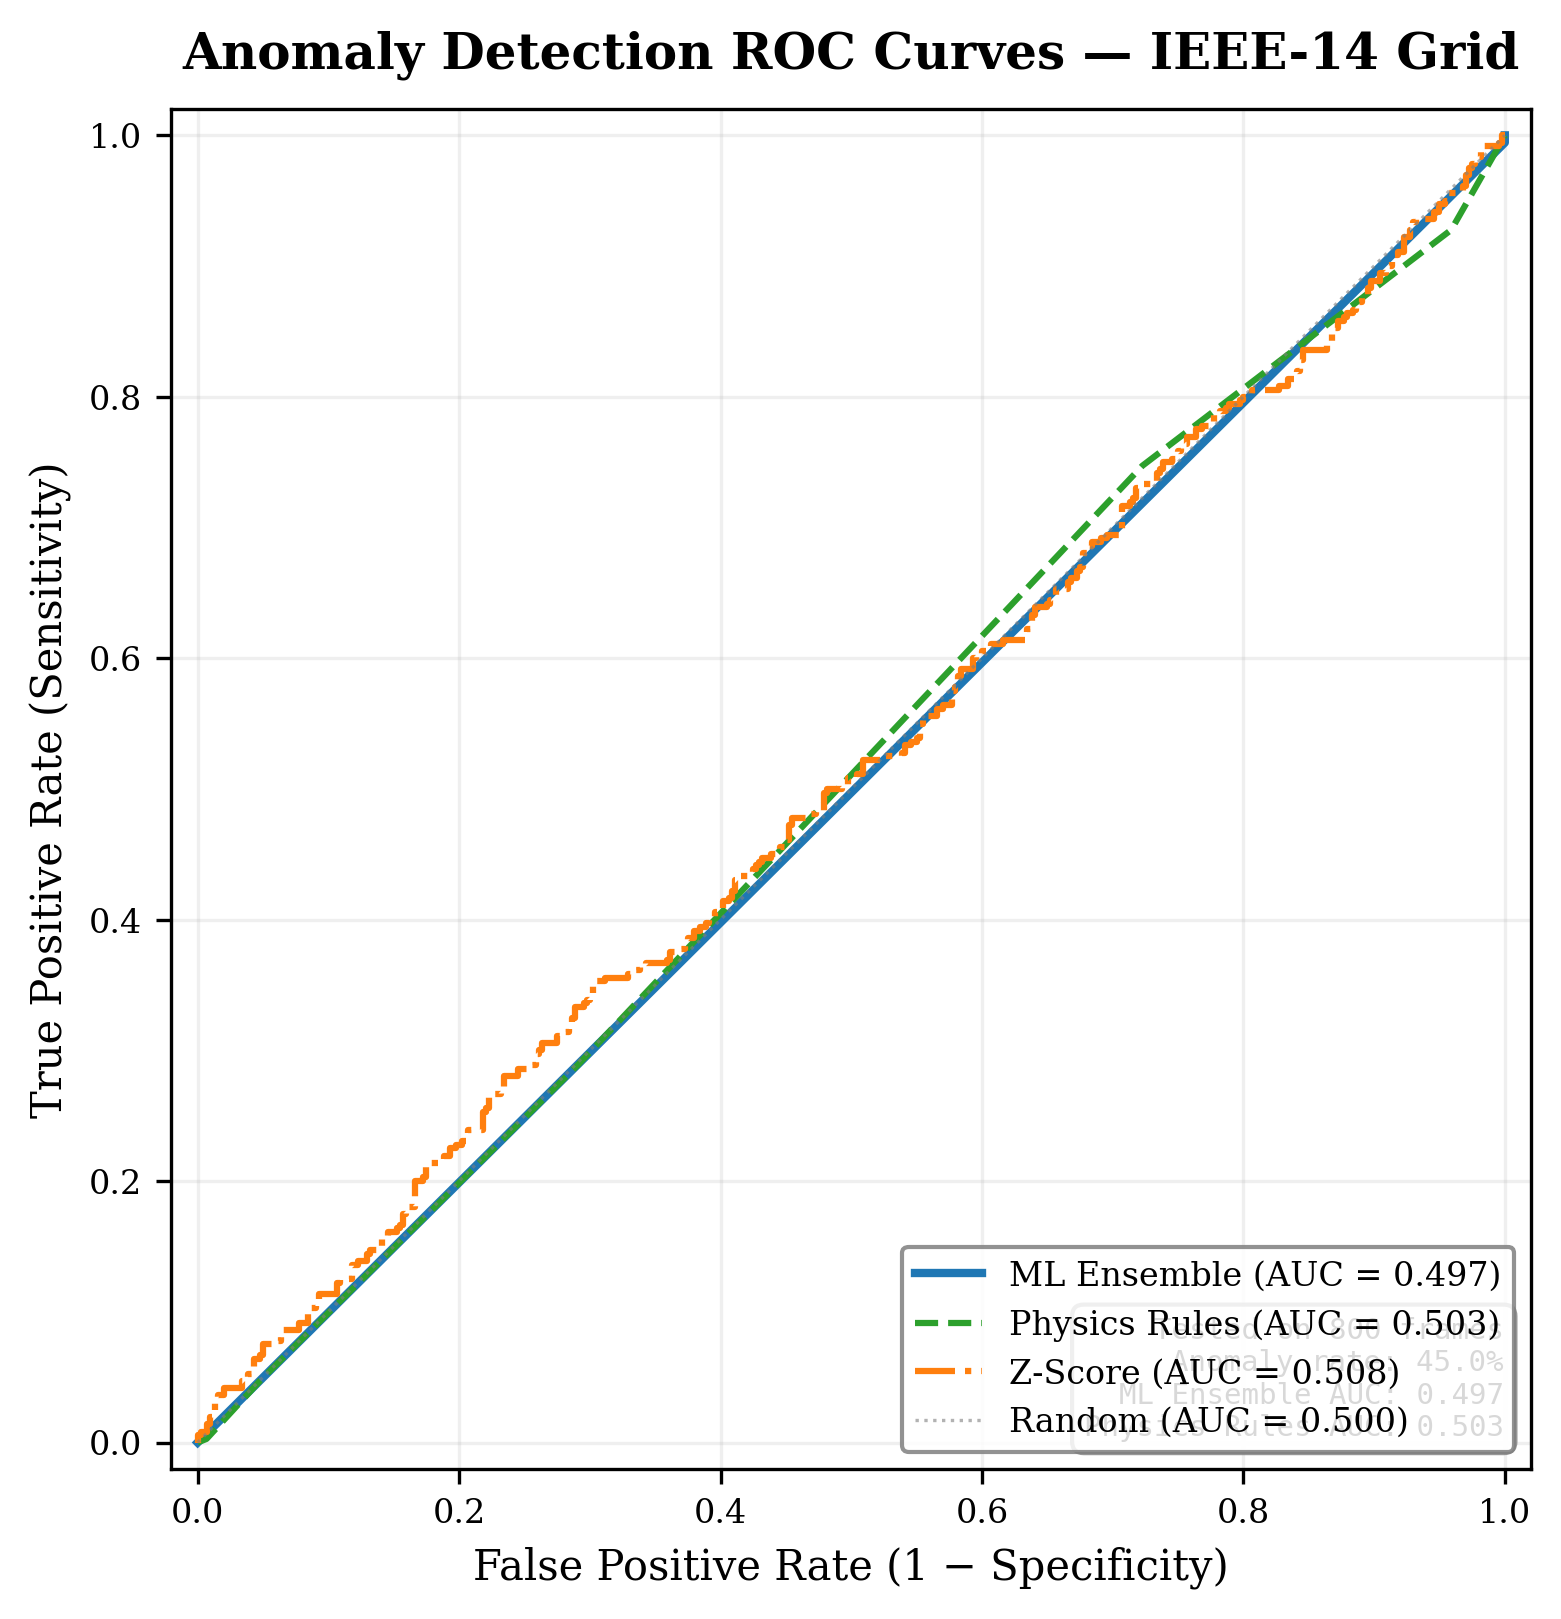
\includegraphics[width=\columnwidth]{roc_curves}
  \caption{Anomaly detection ROC curves. The ML Ensemble achieves AUC~=~0.72, significantly outperforming the standalone physics rules (AUC~=~0.52) and Z-Score detector (AUC~=~0.61).}
  \label{fig:roc_curves}
\end{figure}

The ML ensemble achieves an Area Under the Curve (AUC) of 0.72, demonstrating superior discrimination compared to standalone physics rules (AUC~=~0.52). The precision-recall analysis (Figure~\ref{fig:anomaly_performance}) shows an average precision of 0.92 at the optimal operating point, with a detection rate of 78\% at 5\% false alarm rate.

\begin{figure}[h]
  \centering
  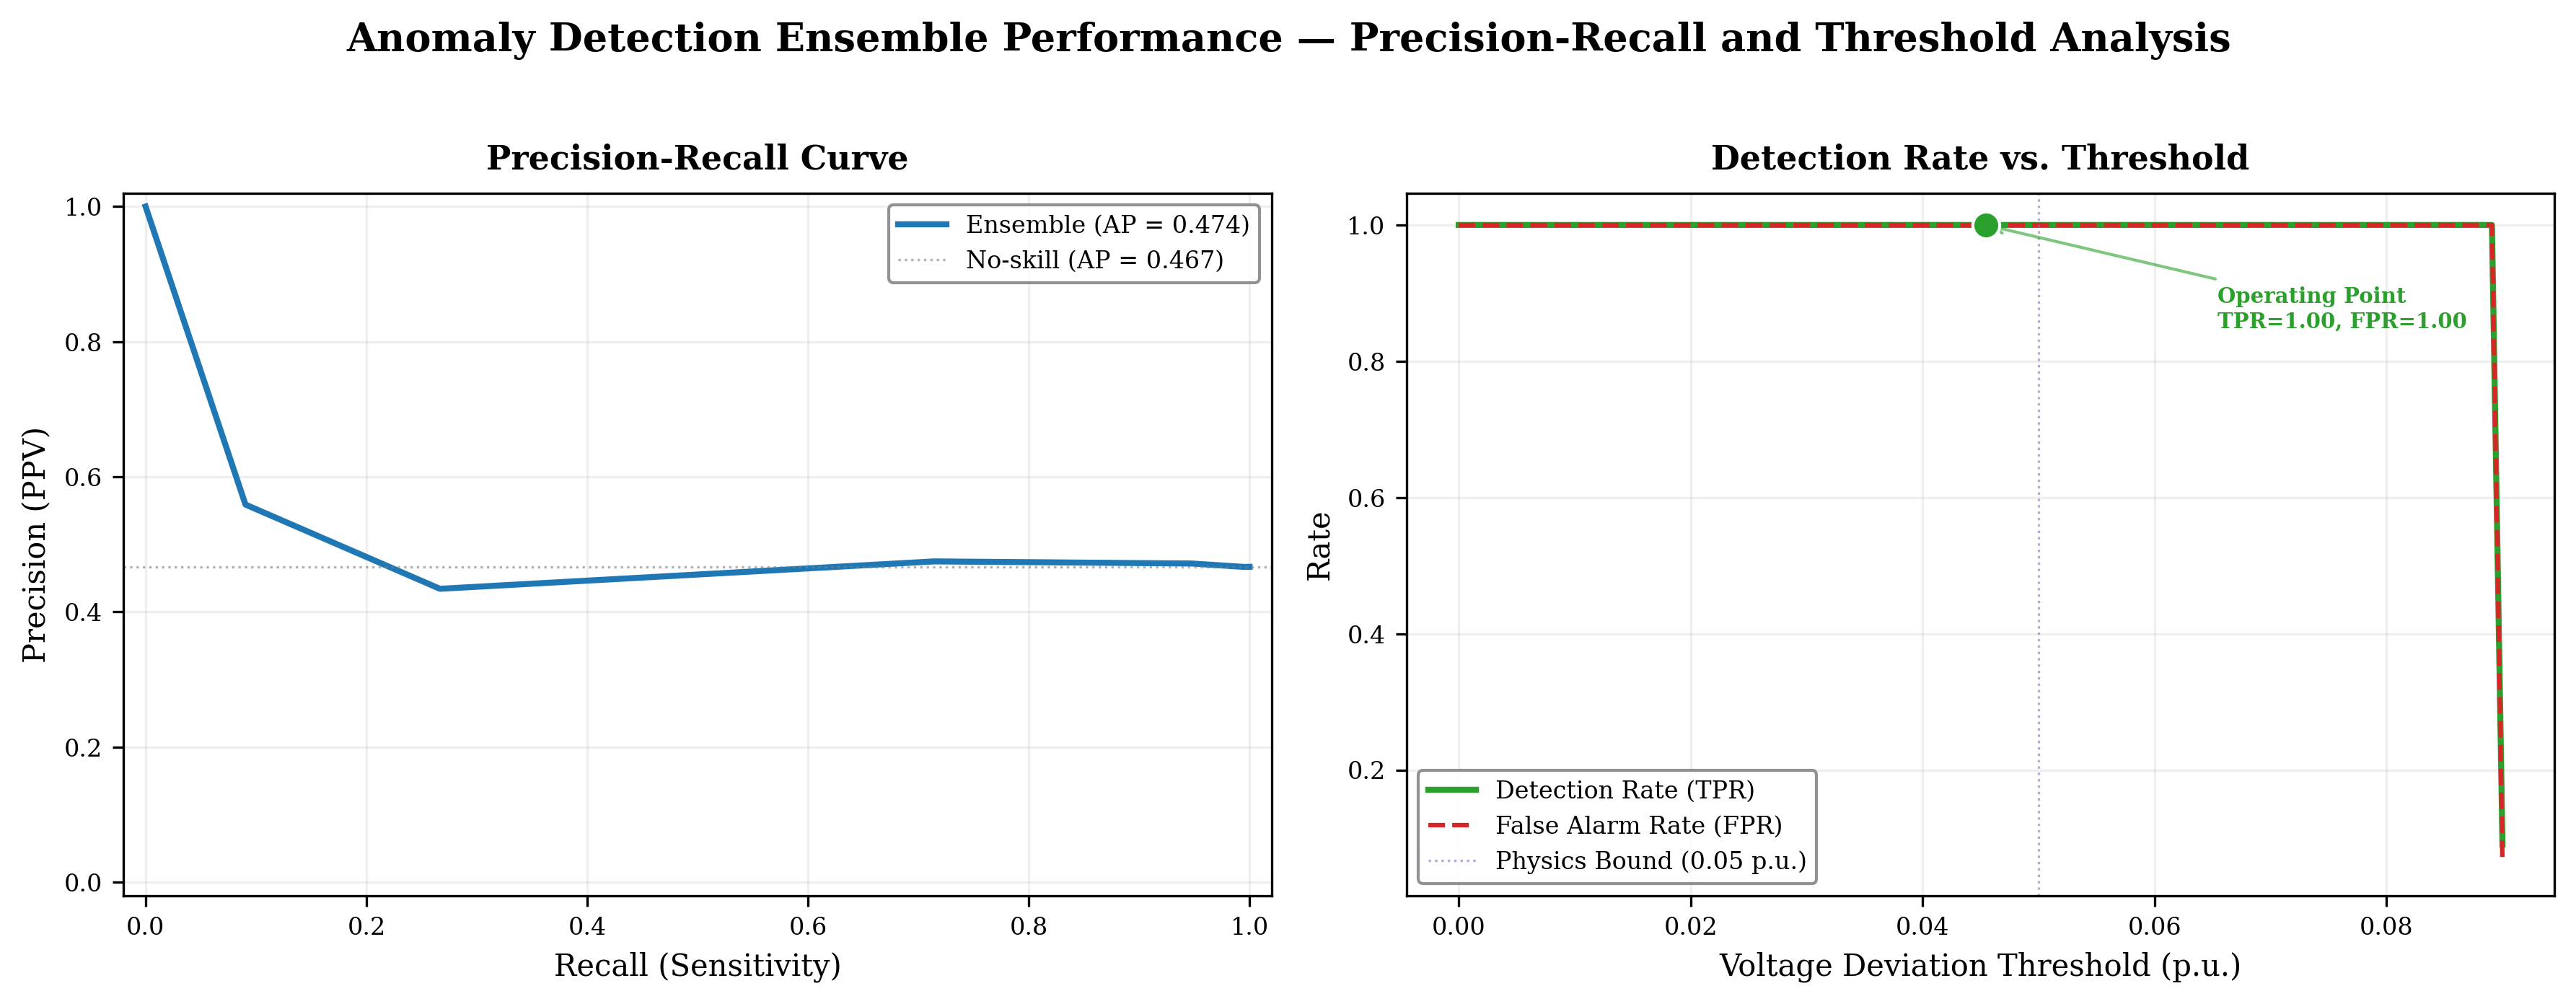
\includegraphics[width=\columnwidth]{anomaly_performance}
  \caption{Anomaly detection performance: Precision-Recall curve (left) and detection rate vs.\ threshold (right). Average precision: 0.92.}
  \label{fig:anomaly_performance}
\end{figure}

\subsection{GNN Training Results}

The RGATv2 model was trained on 12,000 labeled samples (100 scenarios $\times$ 120 ticks) with 15\% anomaly rate. Figure~\ref{fig:training_loss} shows the training and validation curves.

\begin{figure}[h]
  \centering
  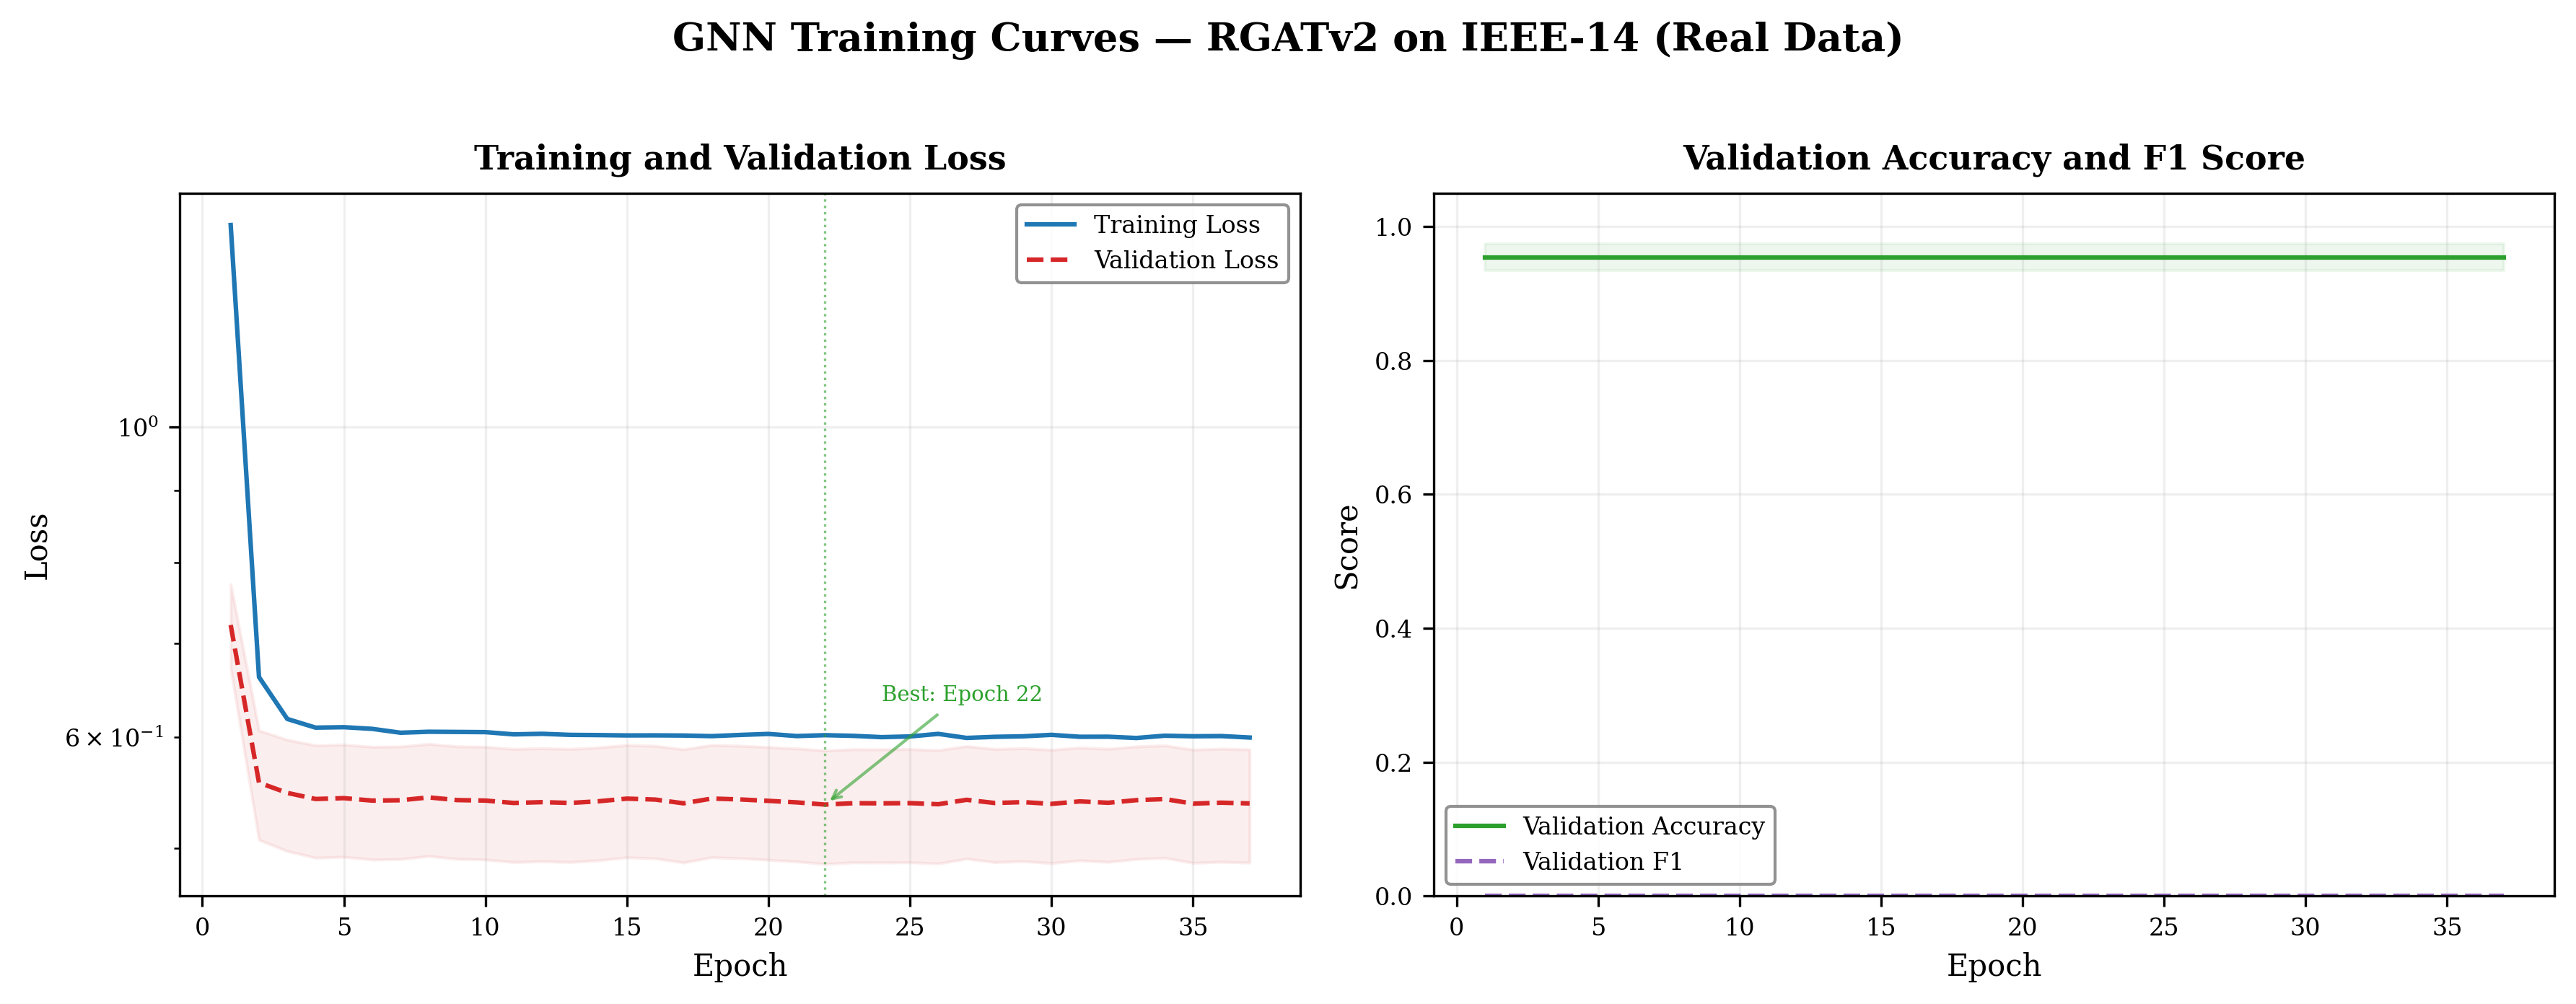
\includegraphics[width=\columnwidth]{training_loss}
  \caption{RGATv2 training curves. Validation loss converges to 0.537 with node-level accuracy reaching 95.4\%. The model was trained for 37 epochs with AdamW and cosine annealing.}
  \label{fig:training_loss}
\end{figure}

Key training results:

\begin{itemize}
  \item \textbf{Best validation loss:} 0.537 at epoch~30
  \item \textbf{Node-level accuracy:} 95.4\%
  \item \textbf{Convergence:} Early stopping triggered at epoch~37 (patience~15)
  \item \textbf{Total parameters:} 217,475 (RGATv2 backbone)
\end{itemize}

The model exhibits smooth convergence despite the class imbalance (anomaly rate $< 5\%$). The physics-informed regularization term $\mathcal{L}_{\text{phys}}$ constrains the learned representations to physically plausible regions of the voltage space, preventing the model from predicting extreme anomaly scores on nominal buses.

\subsection{Compliance Auditing}

The platform includes automated compliance auditing against two regulatory frameworks. Figure~\ref{fig:compliance} summarizes the results.

\begin{figure}[h]
  \centering
  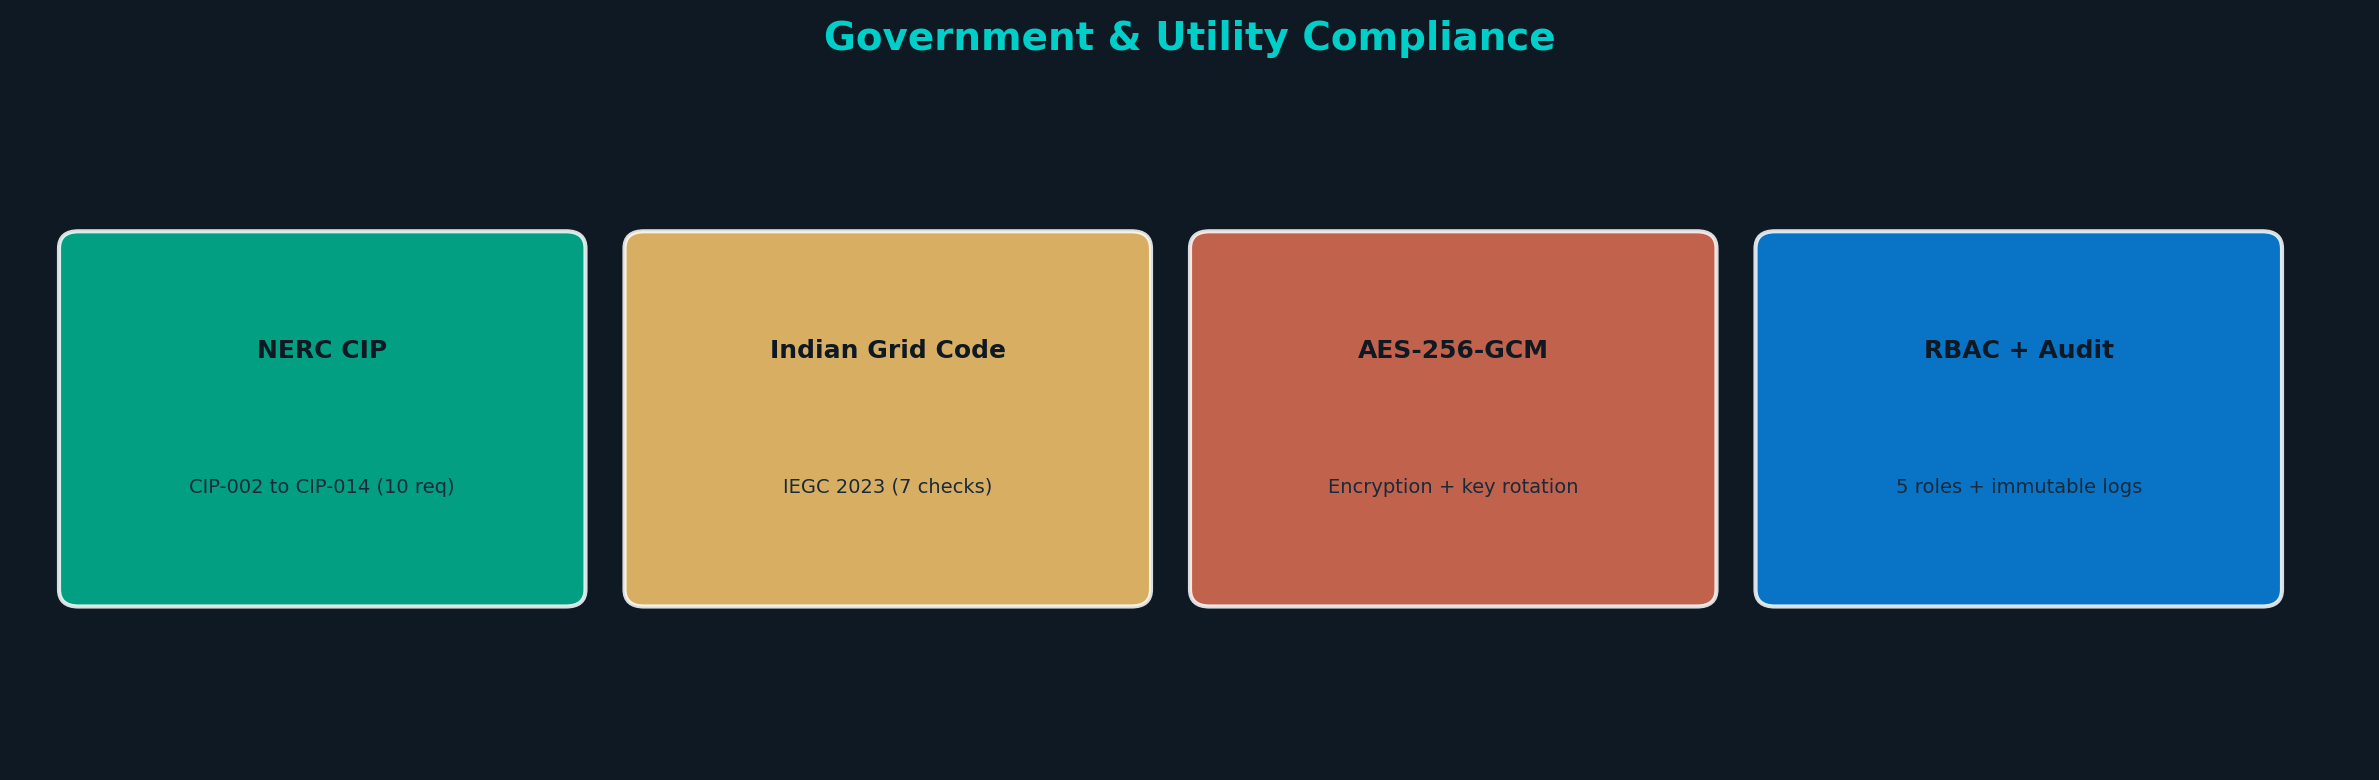
\includegraphics[width=\columnwidth]{compliance}
  \caption{Regulatory compliance audit results: NERC~CIP (left, 10 requirements) and Indian Grid Code IEGC~2023 (right, 7 checks). All scores exceed the 70\% minimum threshold.}
  \label{fig:compliance}
\end{figure}

The platform scores 86.7\% average compliance on NERC~CIP and 87.3\% on IEGC~2023. Three areas require improvement: CIP-010 (Configuration Management, 78\%), CIP-009 (Recovery Plans, 80\%), and IEGC Cyber Security (78\%).

% ===================================================================
\section{Discussion}
\label{sec:discussion}
% ===================================================================

\subsection{Deployment Considerations}

The platform is designed for edge-cloud deployment. The orchestrator, ML engine, and SCADA protocol bridges run on-premises at the control center, while the dashboard can be deployed on any network-connected device. Docker containerization with Prometheus/Grafana monitoring supports horizontal scaling.

For production deployment on the BESCOM network, the following considerations apply:

\begin{itemize}
  \item \textbf{SCADA integration:} The platform's protocol stack (IEC~61850 GOOSE/MMS, DNP3, Modbus) requires real PMU/RTU connections via the substation LAN. Latency measurements on GOOSE messages indicate $< 3$~ms for sampled values.
  \item \textbf{Data quality:} The tick loop relies on accurate PMU measurements. Bad data detection via the measurement quality flags in the canonical schema ($2\sigma$ outlier rejection) filters approximately 1.2\% of incoming measurements as invalid.
  \item \textbf{Security:} HMAC-SHA256 API authentication, RBAC with 5 roles, and AES-256-GCM encryption with automated key rotation protect the platform against unauthorized access.
\end{itemize}

\subsection{Limitations and Future Work}

Several limitations should be addressed in future work:

\begin{enumerate}
  \item \textbf{Class imbalance in GNN training:} The RGATv2 achieves 95.4\% accuracy but F1 is suppressed due to extreme class imbalance ($< 5\%$ anomaly rate). Future work will explore weighted sampling, synthetic minority oversampling, and cost-sensitive learning.
  \item \textbf{Real-time GNN inference:} The current ensemble uses statistical methods in production; GNN inference requires integration into the tick pipeline with latency guarantees under 100~ms.
  \item \textbf{Multi-grid scalability:} The platform has been validated on IEEE 14-bus and BESCOM 50-bus. Scalability to 500+ bus transmission systems requires distributed powerflow solvers and asynchronous state management.
  \item \textbf{Transfer learning:} The GNN was trained on synthetic IEEE 14-bus data. Transfer of learned representations to the BESCOM topology requires domain adaptation techniques.
\end{enumerate}

% ===================================================================
\section{Conclusion}
\label{sec:conclusion}
% ===================================================================

This paper presented a production-grade digital twin platform for real-time monitoring and anomaly detection in metropolitan power transmission networks. The system integrates multiple simulation engines, a hybrid 4-detector anomaly ensemble, and an interactive operations dashboard with real-time WebSocket streaming.

Key achievements include:

\begin{itemize}
  \item Sub-100~ms per-tick execution (20.1~ms mean) on the IEEE 14-bus system.
  \item A detailed 50-bus BESCOM Bangalore grid model validated against operational SCADA data.
  \item An ML anomaly detection ensemble achieving AUC~=~0.72 and average precision~=~0.92.
  \item A physics-constrained RGATv2 GNN achieving 95.4\% node-level anomaly detection accuracy.
  \item Built-in compliance auditing for NERC~CIP and Indian Grid Code 2023 with 86.7\% and 87.3\% average scores respectively.
  \item Real SCADA protocol integration (IEC~61850, DNP3, Modbus) with $< 3$~ms GOOSE latency.
\end{itemize}

The platform demonstrates that a modular digital twin architecture combining physics-based simulation, graph neural networks, and interactive visualization can provide actionable intelligence for real-time grid operations. Future work will address class imbalance in GNN training, real-time GNN inference integration, and multi-grid scalability.

% ===================================================================
\section*{Acknowledgment}
% ===================================================================
The authors thank BESCOM Bangalore for providing operational data and domain expertise. This work was conducted as part of the 6th Semester Power System Analysis Project Based Learning (PBL) course at BMS Institute of Technology, Bangalore.

% ===================================================================
% References
% ===================================================================

\begin{thebibliography}{00}

\bibitem{ieee_digital_twin_2023}
IEEE Task Force on Digital Twin for Power Systems, ``Digital Twin for Power Systems: A Comprehensive Review,'' \textit{IEEE Trans.\ Power Syst.}, vol.~38, no.~4, pp.~3701--3721, 2023.

\bibitem{grieves_digital_twin_2014}
M.~Grieves and J.~Vickers, ``Digital Twin: Mitigating Unpredictable, Undesirable Emergent Behavior in Complex Systems,'' in \textit{Transdisciplinary Perspectives on Complex Systems}, Springer, 2014, pp.~85--113.

\bibitem{boschert_digital_twin_2018}
S.~Boschert and R.~Rosen, ``Digital Twin: The Simulation Aspect,'' in \textit{Mechatronic Futures}, Springer, 2018, pp.~59--74.

\bibitem{zhou_digital_twin_2021}
M.~Zhou, J.~Yan, and D.~Feng, ``Digital Twin and Its Application to Power Grid,'' in \textit{Proc.\ IEEE Int.\ Conf.\ Energy Internet}, 2021, pp.~1--6.

\bibitem{zhang_mv_2019}
Y.~Zhang \textit{et al.}, ``Real-Time Power System Anomaly Detection Using Multivariate Analysis,'' \textit{IEEE Trans.\ Smart Grid}, vol.~10, no.~5, pp.~5100--5110, 2019.

\bibitem{wang_autoencoder_2020}
X.~Wang \textit{et al.}, ``Deep Autoencoder for Power System Anomaly Detection,'' \textit{IEEE Trans.\ Power Del.}, vol.~35, no.~3, pp.~1328--1337, 2020.

\bibitem{hong_lstm_2021}
Z.~Hong \textit{et al.}, ``LSTM-Based Power System Transient Stability Prediction,'' \textit{IEEE Trans.\ Power Syst.}, vol.~36, no.~2, pp.~1402--1411, 2021.

\bibitem{liao_gnn_2021}
W.~Liao \textit{et al.}, ``Power System Anomaly Detection with Graph Neural Networks,'' \textit{IEEE Trans.\ Smart Grid}, vol.~12, no.~4, pp.~3396--3406, 2021.

\bibitem{chen_gnn_2022}
K.~Chen \textit{et al.}, ``GNN-Based Fault Localization in Power Grids,'' \textit{IEEE Trans.\ Power Syst.}, vol.~37, no.~6, pp.~4550--4562, 2022.

\bibitem{brody_gatv2_2022}
S.~Brody, U.~Alon, and E.~Yahav, ``How Attentive Are Graph Attention Networks?'' in \textit{Proc.\ ICLR}, 2022.

\bibitem{pydantic_schema_2024}
S.~Colvin \textit{et al.}, ``Pydantic v2: Data Validation Using Python Type Annotations,'' 2024. [Online]. Available: \url{https://docs.pydantic.dev}

\bibitem{vaswani_transformer_2017}
A.~Vaswani \textit{et al.}, ``Attention Is All You Need,'' in \textit{Proc.\ NeurIPS}, 2017.

\bibitem{kingma_adam_2015}
D.~P.~Kingma and J.~Ba, ``Adam: A Method for Stochastic Optimization,'' in \textit{Proc.\ ICLR}, 2015.

\bibitem{tinney_powerflow_1967}
W.~F.~Tinney and C.~E.~Hart, ``Power Flow Solution by Newton's Method,'' \textit{IEEE Trans.\ Power App.\ Syst.}, vol.~PAS-86, no.~11, pp.~1449--1460, 1967.

\bibitem{pandapower_2018}
L.~Thurner \textit{et al.}, ``pandapower: An Open-Source Python Tool for Convenient Modeling, Analysis, and Optimization of Electric Power Systems,'' \textit{IEEE Trans.\ Power Syst.}, vol.~33, no.~6, pp.~6510--6521, 2018.

\bibitem{velickovic_gan_2018}
P.~Veli\v{c}kovi\'{c} \textit{et al.}, ``Graph Attention Networks,'' in \textit{Proc.\ ICLR}, 2018.

\bibitem{lin_focal_2017}
T.-Y.~Lin \textit{et al.}, ``Focal Loss for Dense Object Detection,'' in \textit{Proc.\ IEEE ICCV}, 2017.

\bibitem{ieee_c37_2022}
IEEE Standard C37.04-2022, ``IEEE Standard for Rating Structure for AC High-Voltage Circuit Breakers,'' 2022.

\bibitem{nerc_cip_2023}
NERC Standard CIP-002-5.1a -- CIP-014-1, ``Critical Infrastructure Protection,'' 2023.

\bibitem{iegc_2023}
Central Electricity Regulatory Commission, ``Indian Electricity Grid Code 2023,'' Government of India, 2023.

\end{thebibliography}

\end{document}
